\chapter{ОСНОВНЫЕ ПОНЯТИЯ И ОБЗОР ЛИТЕРАТУРЫ }\label{chap1}

\bigskip
Врезку пока не делал
\bigskip
%Первая глава всегда посвящена обзору литературы. В начале каждой главы необходимо написать небольшую аннотацию о содержании главы (так называемая \textit{врезка}). Например:
%
%В настоящей глава формулируются основные понятия, используемые в диссертации. Приводится классификация (согласно работе \cite{GabasovKirillovaPU}) принципов управления, используемых в современной теории управления. Объясняется принцип управления в режиме реального времени в применении к реализации оптимальных обратных связей в задачах оптимального управления с конечным горизонтом планирования \cite{GabasovDmitrukKirillova15a} и в применении к задачам стабилизации нелинейных объектов согласно теории  управления по прогнозирующей модели \cite{Mayne}.

%%%%%%%%%%%%%%%%%%%%%%%%%%%%%%%%%%%%%%%%%%%%%%%%%%%%%%%%%%%%%%%%%%%%%%%%%%%%%%%%
\section{Задачи оптимального управления}\label{1sec:optimal-control}
%%%%%%%%%%%%%%%%%%%%%%%%%%%%%%%%%%%%%%%%%%%%%%%%%%%%%%%%%%%%%%%%%%%%%%%%%%%%%%%%
Задача оптимального управления формируется из пяти составляющих: временного интервала, математической модели, класса управлений и ограничений на них, ограничений на фазовую траекторию и критерия качества.


\textbf{1) Временной интервал.} По временному интервалу задачи оптимального управления разделяются на непрерывные, рассматриваемые на некотором промежутке времени $T = [t_0,~ t_f]$, и дискретные, где используются дискретные моменты времени $T_h = \{t_0,~ t_0 + h, \ldots , t_f - h \}, ~h = \dfrac{t_f-t_0}{N}, ~N \in \mathbb{N}$, то есть, например, если $t \in [s,~s+h[ ,~s \in T_h$, то дискретное управление $ u(t) = u(s) $.
Выделяют задачи с фиксированным и нефиксированном временем окончания динамического процесса, а также задачи на бесконечном интервале.


\textbf{2) Математическая модель.} Динамический процесс обычно моделируется дифференциальными
\[ \dot x(t) = f(x(t), u(t), t) \]
или разностными уравнениями
\[ x(k + 1) = f(x(k), u(k), k), k = 0, 1, ...\]
где $n$-вектор $x$ называется состоянием системы, $r$-вектор $u$ называется управлением, функция $f : \mathbb{R}^n \times \mathbb{R}^r \times \mathbb{R} \to \mathbb{R}^n$ задана.


\textbf{3) Класс управлений и ограничения на них.} Для непрерывного
процесса управления четко указывается класс функций, из которого выбираются управления. Кроме класса доступных управлений задается множество $ U \subset \mathbb{R}^r $ --- множество допустимых значений управления. Как правило $U$ --- компакт в  $\mathbb{R}^r $.


\begin{definition}  Кусочно-непрерывная (дискретная, измеримая
и т.д.) функция $  u(\cdot) = (u(t),~ t \in [t_0,~ t_f])$ называется доступным управлением, если $u(t) \in U,~ t \in [t_0, ~t_f]$.
\end{definition}


\textbf{4) Ограничения на фазовую траекторию. } Ограничения на переменные состояния могут накладываться в начальный момент времени $t_0$:
\[x(t_0) \in X_0;\]
в конечный момент времени $t_f$, такие ограничения называются терминаль-
ными:
\[x(t_f) \in X_f;\]
в изолированные моменты $t_i \in [t_0,~ t_f], ~i = 1, m$, из промежутка управления --- промежуточные фазовые ограничения
\[X(t_i) \in X_i, ~i = 1, m\]
на всем промежутке управления --- фазовые ограничения
\[x(t) \in X(t), ~ t \in [t_0,~ t_f]\]
где $X_0,~ X_f,~ X_i, ~i = 1, m, ~X(t),~ t \in [t_0,~ t_f]$, --- заданные множества пространства состояний.


\begin{definition}   Доступное управление $  u(\cdot) = (u(t),~ t \in [t_0,~ t_f])$ называется допустимым (или, программой), если оно порождает траекторию $  x(\cdot) $, удовлетворяющую всем ограничениям задачи.
\end{definition}


\textbf{5) Критерий качества. }
Множество допустимых управлений, как правило, содержит более одного элемента, поэтому возникает необходимость сравнивать их между собой. Для этого вводится функционал $ J(u)$, называемый критерием качества, и выбирается операция минимизации или максимизации этого функционала, результат которой определяет наилучшее(оптимальное) управление.
В теории оптимального управления различают четыре типа критериев
качества: Майера, Больца, Лагранжа, задачи быстродействия. Все 4 критерия качества эквивалентны между собой.


Для примера выпишем критерий качества типа Майера(териминальный критерий):
\[ J(u) = \varphi (x(t_f)). \]


Объектом исследований в настоящей работе будут непрерывные задачи оптимального управления линейными нестационарными системами с линейным терминальным ограничением и критерием качества:


\begin{equation}
    J(u) = c'x(t_f) \to max,
\end{equation} 
\[ \dot x = A(t)x + B(t)u,~~~x(t_f) \in X_f,~~~t \in T = [t_0,~t_f]\]

Задачи будут исследоваться в классе дискертных управляющих воздействий (см. разд. 1.3).


%%%%%%%%%%%%%%%%%%%%%%%%%%%%%%%%%%%%%%%%%%%%%%%%%%%%%%%%%%%%%%%%%%%%%%%%%%%%%%%%
\section{Программные и позиционные решения}
%%%%%%%%%%%%%%%%%%%%%%%%%%%%%%%%%%%%%%%%%%%%%%%%%%%%%%%%%%%%%%%%%%%%%%%%%%%%%%%%
Рассмотрим задачу оптимального управления:


\begin{equation}\label{simpleEq_2_1}
    c'x(t_f) \to max,~~~\dot x = A(t)x + B(t)u,~~~x(t_0) = x_0,
\end{equation} 
\[ x(t_f) \in X_f,~~~u(t) \in U, ~~~t \in T = [t_0,~t_f]\]


Пусть ее модель управляема в классе дискретных управляющих воздействий:
\[u(t) \equiv u(\tau), ~~~t \in [\tau, ~\tau + h[,~~~ \tau \in T_h = \{t_0,~ t_0 - h, \dots ,~ t_f - h\} \]


\begin{definition}   Программа $u^0(t), ~t \in T,$ называется программным решением задачи (\ref{simpleEq_2_1}) (оптимальной программой), если на соответствующей ей траектории $x^0(t), ~t \in T,$ выполняется равенство $c'x^0(t_f) = \max_u c'x(t_f) $.
\end{definition}


Приведем задачу (\ref{simpleEq_2_1}) к набору задач, зависящих от скаляра $\tau \in T_h = \{t_0,~ t_0 - h, \dots ,~ t_f\}$:


\begin{equation}\label{simpleEq_2_2}
    c'x(t_f) \to max,~~~\dot x = A(t)x + B(t)u,~~~x(\tau) = z,
\end{equation} 
\[ x(t_f) \in X_f, ~~~u(t) \in U ,~~~t \in T(\tau) = [\tau,~t_f]\]


Пусть $ u^0(t|\tau, z),~ t \in T(\tau), $ --- оптимальная программа задачи (\ref{simpleEq_2_2}) для позиции $(\tau, z)$; $~X_\tau$ --- множество состояний $z$, для которых в момент $\tau$ существуют программные решения.


\begin{definition}   Функиция
\[ u^0(\tau, z) = u^0(\tau|\tau, z),~~~ z \in X_\tau,~~~ \tau \in T_h,\]
называется позиционным решением задачи (\ref{simpleEq_2_2}) (оптимальной обратной связью).
\end{definition}
 

Управление называется программным, если оно регулируется программно, строго, без динамического наблюдения за состоянием объекта и контроля воздействия на него, то есть базируясь только на априорных оценках. В случае позиционного управления кроме априорных оценок для формирования управляющего воздействия используются текущие данные.
	
	
Программное управление редко применяется на практике, так как со временем, из-за изначальной неточности математической модели и построения обратных связей, а также из-за действия в процессе управления неизвестных возмущений, накапливается общая пограешность вычислений. 


Программное и позиционное управления следуют одному из трех принципов управления: по разомкнутому контуру, по замкнутому контуру, в реальном времени. Программные управления исполняются на разомкнутом контуре, а позиционные --- на замкнутом и в реальном времени. При создании систем управления по замкнутому контуру используются связи 3-х типов: прямые, обратные и комбинированные (Рис. \ref{fig:1_2_1}). С их помощью получают замкнутые системы управления.


\begin{figure}[h]
	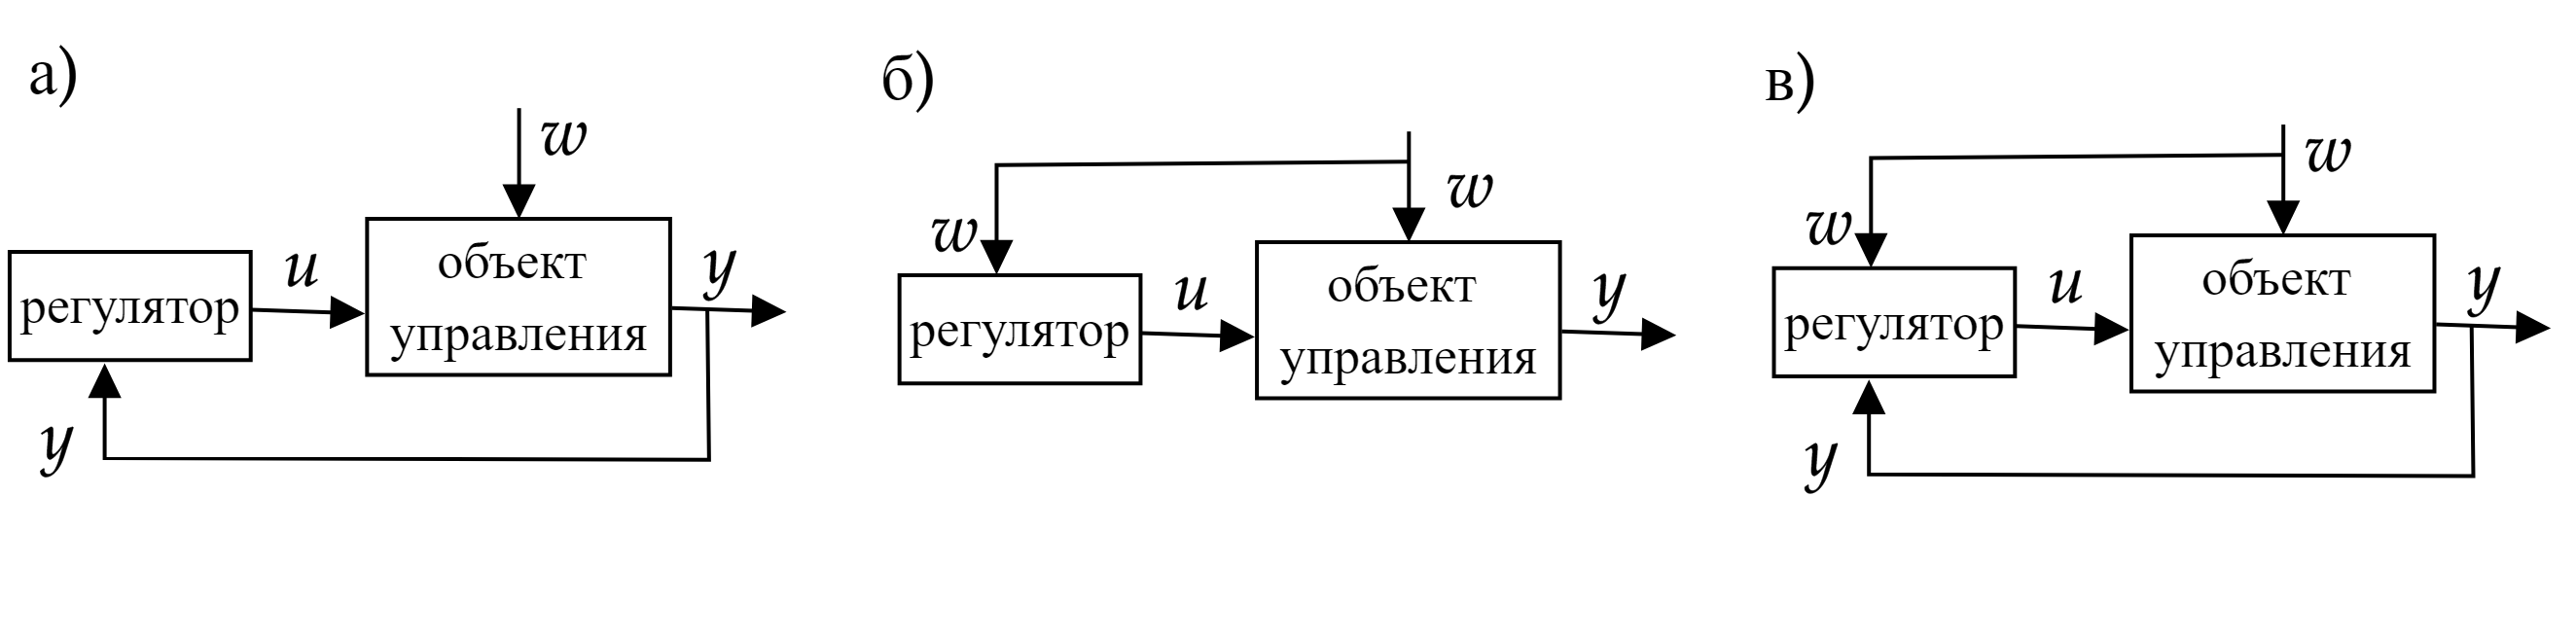
\includegraphics[width=\linewidth]{1_2_1.png}
  	\caption{а) обратная связь; б) прямая связь; в) комбинированная связь}
  	\label{fig:1_2_1}
\end{figure}


В системах реального времени данные связи не строятся явно. Нужные для управления текущие значения связей вычисляются по ходу каждого процесса управления вычислительными устройствами.


%Системы управления в реальном времени изображаются так же, как замкнутые системы. Разница между ними состоит в реализации связей: в системах управления в реальном времени они осуществляются программно, гибко, а в замкнутых системах --- аппаратно, жестко.


Замкнутые системы управления и системы управления в реальном времени называют автоматическими и автоматизированными соответственно.


%%%%%%%%%%%%%%%%%%%%%%%%%%%%%%%%%%%%%%%%%%%%%%%%%%%%%%%%%%%%%%%%%%%%%%%%%%%%%%%%
\section{Управление в реальном времени}\label{1_3}
%%%%%%%%%%%%%%%%%%%%%%%%%%%%%%%%%%%%%%%%%%%%%%%%%%%%%%%%%%%%%%%%%%%%%%%%%%%%%%%%


%Для описания принципа управления в реальном времени рассмотрим простейшую задачу оптимального управления:
%
%
%\begin{equation}\label{simpleEq1}
%    c'x(t_f) \to max,~~~\dot x = A(t)x + B(t)u,~~~x(t_0) = x_0,
%\end{equation} 
%\[ x(t_f) \in X_f = \{x \in R^n :g_* \leq Hx \leq g^*\},\]
%\[u(t) \in U = \{u \in R^r :u_* \leq u \leq u^*\},~~~t \in T = [t_0,~t_f] \]
%
%
%Задача (\ref{simpleEq1}) будет исследоваться в классе дискретных управляющих воздействий:
%\[u(t) \equiv u(\tau), ~~~t \in [\tau, ~\tau + h[,~~~ \tau \in T_h = \{t_0,~ t_0 - h, \dots ,~ t_f - h\} \]
%
%
%Приведем ее к набору задач, зависящих от скаляра $\tau \in T_h = \{t_0,~ t_0 - h, \dots ,~ t_f\}$:
%
%
%\begin{equation}\label{simpleEq2}
%    c'x(t_f) \to max,~~~\dot x = A(t)x + B(t)u,~~~x(\tau) = z,
%\end{equation} 
%\[ x(t_f) \in X_f, ~~~u(t) \in U ,~~~t \in T(\tau) = [\tau,~t_f]\]
%
%
%Пусть $ u^0(t|\tau, z),~ t \in T(\tau), $ --- оптимальная программа задачи (\ref{simpleEq2}) для позиции $(\tau, z)$; $~X_\tau$ --- множество состояний $z$, для которых существуют программные решения. Функиция
%\[ u^0(\tau, z) = u^0(\tau|\tau, z),~~~ z \in X_\tau,~~~ \tau \in T_h,\]
%называется оптимальной обратной связью.


В описываемом принципе управления обратная связь не строится. Управляющее воздействие $ u^*(\tau) $ создается в процессе управления при каждом $ \tau \in T_h $ за время $ s(\tau)$, не превосходящее $h$. Устройство, способное выполнять эту работу, называется оптимальным регулятором, реализующим оптимальную обратную связь. 


%%%%%%%%%%%%%%%%%%%%%%%%%%%%%%%%%%%%%%%%%%%%%%%%%%%%%%%%%%%%%%%%%%%%%%%%%%%%%%%%
\section{Численные методы решения задач оптимального управления и программные средства}
%%%%%%%%%%%%%%%%%%%%%%%%%%%%%%%%%%%%%%%%%%%%%%%%%%%%%%%%%%%%%%%%%%%%%%%%%%%%%%%%
(Не понял, что требуется написать)



........

\bigskip
Краткие выводы пока не делал 
%Каждая глава завершается краткими выводами. Разумный способ написания выводов --- переписать (это значит использовать те же мысли, но не копировать фразы!) в утвердительной форме (рассмотрено, получено и т.д.) то, что написано во врезке. 
